\chapter{AccessibleEPUB Editor}
\label{ch:AccessibleEPUB Editor}

The AccessibleEPUB editor will be presented with each Windows form covering a separate section.

\section{Requirements}

There are a variety of requirements which have to be fulfilled the editor. Most importantly, it has easy to use and not require any programming knowledge to use, except for LaTeX code for equations. If no equations are needed in the document, then there must be programming ability asked of the user. 

\section{Programming language}

The first question was in which programming language should the editor be implemented in. C\# and Java were picked early as the two main options, as both of them are object oriented and natively support forms. Furthermore, both support the ability to make the programs themselves accessible for blind users. C\# has several accessibility properties, like AccessibilityDescription and AccessibilityName, which are passed to the screen reader. Java uses the Java Accessibility Bridge which makes it accessible to screen readers. Java is platform independent, and while C\# programs can run on Mac OS and Linux, it relies heavily on Windows and its features. However, Java is not already installed on any operating system, while C\# programs can run on Windows machine with only .NET as prerequisite. The target .NET version of the editor is contained in Windows 10. Therefore the editor was programmed in C\#, as the users were predominantly Windows users and don't have to install prerequisites.

\section{Main window with editor and preview}

\subsubsection{HTML Editor}

\begin{figure}
	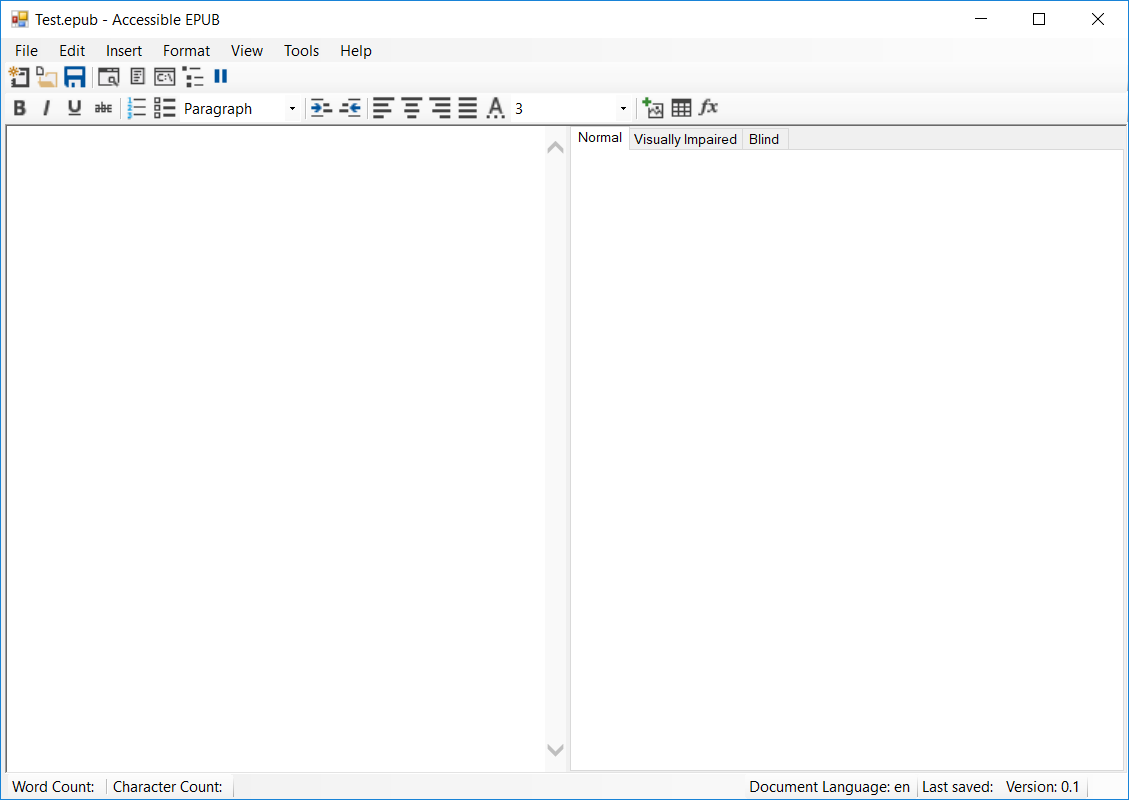
\includegraphics[width=\linewidth]{figures/formJs.png}	
	\caption{Main window with HTML editor and JavaScript switching preview}
	\label{fig:formJs}
\end{figure}

The main window required the most programming and therefore also had its fair share of problems. The first issue was regarding the editor on the left hand side in figure \ref{fig:formJs}. At first a What-You-See-Is-What-You-Get(WYSIWYG) HTML editor was not intended, as it hides semantic information about the EPUB. The initial approach involved editing semantic information of XHTML elements, like images, and changing things like the src, alt, etc. This was still in the early, rough stages and the approach seemed too complicated, so the WYSIWYG editor was chosen instead. 

The second issue was how to implement the WYSIWYG HTML editor. Programming it from scratch would not be possible in the time allocated to a bachelor thesis, as it would involve creating a browser engine. Fortunately, the inbuilt browser in C\#, WebBrowser, allows editing with just a few lines of code. The WebBrowser control is based on Internet Explorer and displays web pages like it. It uses Internet Explorer version 6 as default, which does not display certain CSS properties such as \lstinline|max-width| and cannot display SVGs. To fix this issue, some code has to be run when the form has loaded which determines the Internet Explorer version on the computer and loads the newest one to the HTML editor. After this SVGs and the CSS properties functioned as desired. 

A major issue with the HTML editor is that content written in it is in HTML, while EPUB requires XHTML. While there aren't major differences, there are some small ones such as independent tags like \lstinline|<br>| have to be self closing and written as \lstinline|<br/>| in XHTML. If this is not done the EPUB reader will specify an error. Therefore a tool has to convert the HTML code to XHTML. There are several packages available, one of them being HtmlAgilityPack\footnote{http://html-agility-pack.net/}. It can convert HTML and XHTML and also correct HTML parsing errors such as not closed tags. HtmlAgilityPack functioned well and as expected at first. The resulting code was in XHTML. However, there soon was an error. Many Greek signs, such as the sign "$\wedge$", were displayed as question mark. This meant HtmlAgilityPack could not be used. 

Another available package was TidyManaged\footnote{https://github.com/markbeaton/TidyManaged}, was also used, but it did not convert the code properly to XHTMl. The third attempt involved using SgmlReader\footnote{https://github.com/lovettchris/SgmlReader}, which converts SGML content, like HTML, to XML content, like XHTML. It successfully parsed the HTML and was able to convert mathematical signs properly. It did not create a XML declaration at the top of the document, but this was simpler to solve. A standard XML declaration was just added to the document and the new XHTML document was properly rendered by the browser.


\begin{figure}
	\begin{center}
		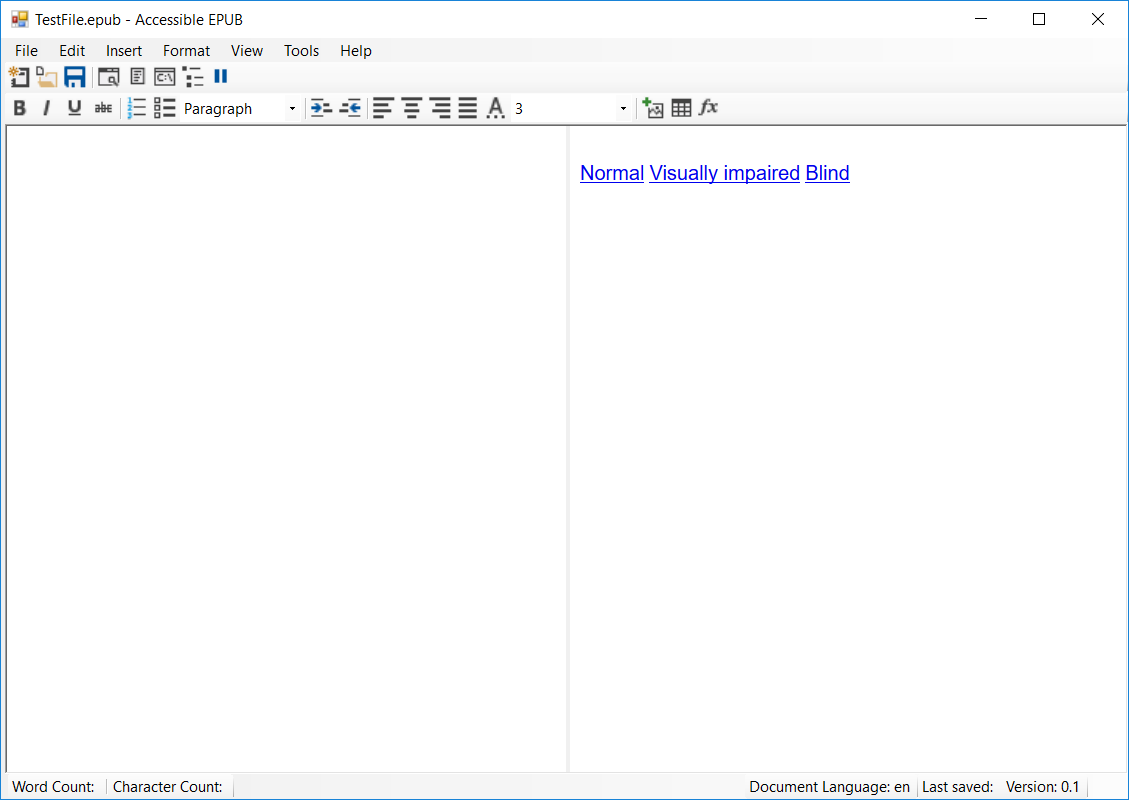
\includegraphics[width=\linewidth]{figures/formCss.png}	
		\caption{Main window with HTML editor and CSS switching preview}
		\label{fig:formCss}
	\end{center}
\end{figure}

\subsubsection{Preview browser}

On the right hand size of the main window is the preview browser. It should display XHTML page in each of three versions(normal, visually impaired, blind). Since the HTML editor uses the WebBrowser control, it would have been easiest to use it on the right side too. However, Internet Explorer is unable to display MathML. Instead of showing the quadratic equation, as shown in figure \ref{fig:quadEquaPng}, it showed figure \ref{fig:IEmathml}. As a result, another browser had to be found. Only two browsers are able properly show MathML, Mozilla Firefox and Safari by Apple. The Firefox engine, Gecko, was chosen as it is open source and had a C\# browser package. After inserting an instance of a \lstinline|GeckoWebBrowser| in the form MathML was displayed properly.

\begin{figure}
	\begin{center}
		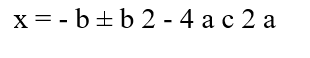
\includegraphics[width=\linewidth/2]{figures/IEmathml.png}	
		\caption{MathML depiction of the quadratic equation in Internet Explorer}
		\label{fig:IEmathml}
	\end{center}
\end{figure}

As seen in figures \ref{fig:formJs} and \ref{fig:formCss}, there is a small difference between the user interface of the JavaScript and CSS versions. The CSS version only uses one browser tab as preview, while the JavaScript version uses three. This is mentioned in chapter \ref{ch:EPUB Document Standard} and is due to the JavaScript version having a separate file named VersionChanger.xhtml, which handles switching versions. In the CSS version the whole content is in one XHTML file. Consequently, the CSS version is very easy to show in the preview. Only the three links shown in figure \ref{fig:css_switch} have to be added to HTML editor content and file is done.

This is much more complicated in the JavaScript version, since the default display style will always be shown. The CSS of the blind and visually impaired version had to be changed. The initial attempt to solve this problem was done by changing the CSS of each browser in a tab and accessing the \lstinline|GeckoStyleSheet| of a browser. Unfortunately, even after changing the \lstinline|GeckoStyleSheet| of a document, it still displayed the default one. An alternative approach consisted of accessing the head(\lstinline|<head>|) of the XHTML document and inserting the CSS there, but this too did not work. These two methods were preferable as they do not have significant input and output (IO) operations. Unfortunately, even slightly altered methods of the two did not function properly. As such an IO intensive approach had to be taken. The XHTML file with the content, \lstinline|Content.XHTML| had to be copied to two new files, \lstinline|BliContent.XHTML| and \lstinline|ImpContent.XHTML| for the blind and visually impaired version, respectively. Then the single line linking the style in XHTML head was replaced with one linking the corresponding CSS. 
Both files are then removed before saving the EPUB and then created again. This is additional overhead, but it was the method which succeeded.

\textcolor{red}{pandoc } %┬▒}

\includegraphics[width=2em]{figures/pandocSigns.png}
